\section{Implementierung}\label{sec:08_05_implementierung}

\subsection{Technologien}
Die Benutzeroberfläche ist eine Single-Page-App, die hauptsächlich in React mit TypeScript geschrieben wurde. TypeScript typisiert JavaScript und ermöglicht die Vorteile einer typisierten Sprache. React Router DOM wurde verwendet, um die Navigation ohne eine Webseitenaktualisierung zu implementieren. Datenfluss und -verwaltung wurden mit Redux und Redux Sagas ermöglicht.  Durch den Einsatz der vordefinierten UI-Elemente von Ant Design und Bootstrap konnten wir eine einheitliche Designsprache beibehalten. Letztlich wurden mit nivo die dynamischen und animierten Grafiken erstellt.


\begin{figure}[hbt!]%
  \centering
  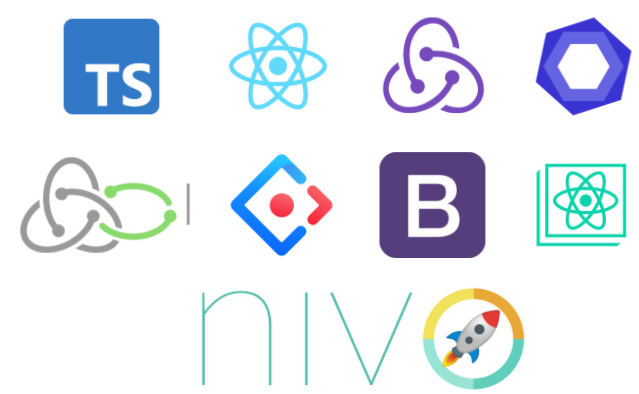
\includegraphics[width=14cm]{images/08-Benutzeroberfläche/08-frontend-framework-icons.PNG}
  \caption{Eine Übersicht über alle verwendeten Technologien, Werkzeuge und Bibliotheken}%
\end{figure}



\subsubsection{React}
React basiert auf dem sogenannten Komponentenmuster (engl. \dq component pattern\dq), in der jedes Element einer Webseite einer \dq stateless\dq Komponente entspricht. \dq Stateless\dq Komponenten sind wiederverwendbare Webseiten Elemente, welche keinen eigenen Status, Daten oder Inhalt besitzen. Sie dienen lediglich für die funktionale Transformationen von Eingabedaten.\cite{ReactDoc} Zudem kann jede Komponente ebenfalls eine Tochterkomponente besitzen.

Die Daten und Komponenten werden von sogenannten Container verwaltet. Ein Container aggregiert die benötigten Komponenten und sorgt für den Datenfluss.

\begin{figure}[hbt!]%
  \centering
  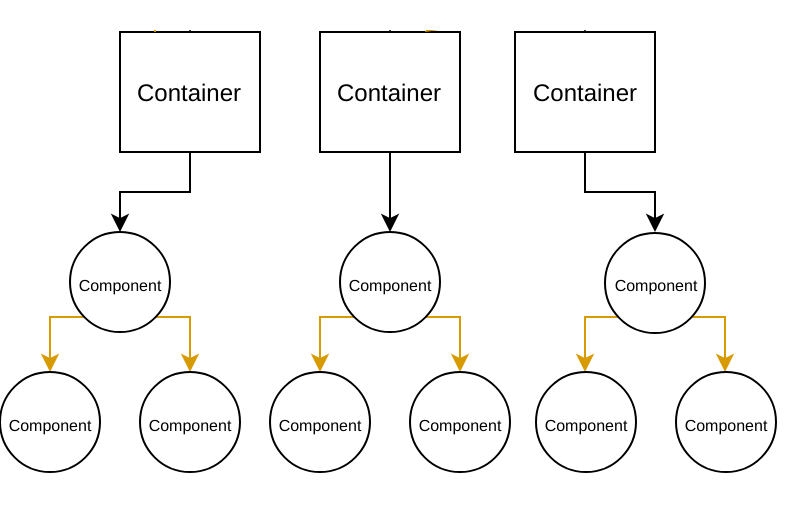
\includegraphics[width=10cm]{images/08-Benutzeroberfläche/08-react-component.PNG}
  \caption{Die Visualisierung vom Datenfluss im Komponentenmuster. Eine Menge von Container besitzen Komponenten welche Daten erhalten und weiter an den Tochterkomponenten übergeben von \cite{itnext18}}%
\end{figure}

\subsubsection{Redux und Redux Sagas}
Redux und Redux-Sagas wurde für den Datenfluss und -verwaltung verwendet. 

Redux dient als ein globaler Speicherort für Informationen. Daher wird Redux oftmals auch als Redux Store bezeichnet. Container greifen auf den Redux Store zum um entweder Daten zu erhalten oder zu verändern. Dabei können Container sogenannte Actions ausführen, um Daten zu erhalten. Mithilfe von Reducer können Daten vorselektiert oder verändert werden. 

\begin{figure}[hbt!]%
  \centering
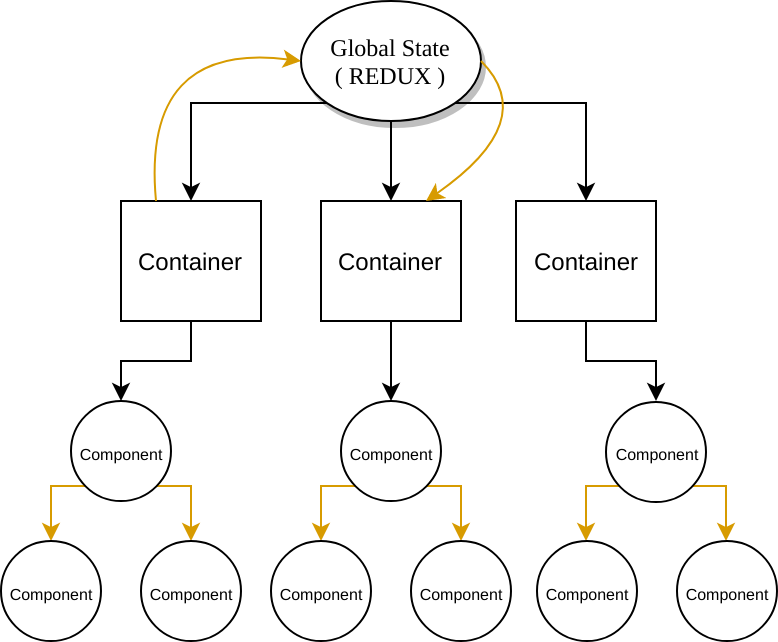
\includegraphics[width=10cm]{images/08-Benutzeroberfläche/08-react-redux.png}
  \caption{Die Visualisierung vom Datenfluss im Komponentenmuster mit Redux von \cite{itnext18}}%
\end{figure}

Die Informationen im Redux Store müssen jedoch erst von einem Server angefordert werden. Dieser Vorgang ist jedoch asynchron und gibt keine Informationen über den Status des Prozesses zurück. Beispielsweise es ist nicht bekannt ob der Server die Daten verarbeitet oder ob der Prozess fehlgeschlagen ist. Der Anwender hingegen möchte wissen, ob Daten gerade verarbeitet werden. Um dies zu ermöglichen, wurde Redux-Sagas eingesetzt. Redux-Sagas ist eine Middleware, die sich zwischen der Benutzeroberfläche und dem Redux Store befindet. Wenn die Benutzerfläche eine Action ausführt, wird die Middleware Daten vom Server anfordern und dem Reducer weitergeben. Der Reducer wiederum bearbeitet die Daten und speichert sie im Redux Store. 

\begin{figure}[hbt!]%
  \centering
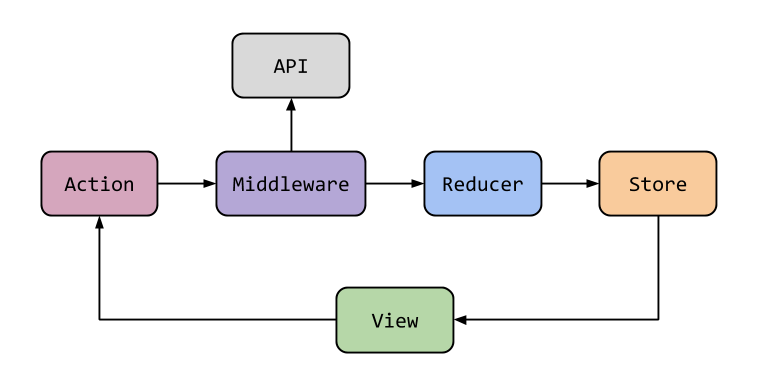
\includegraphics[width=10cm]{images/08-Benutzeroberfläche/08-redux-middleware-diagram.png}
  \caption{Die Visualisierung vom Datenfluss mit Redux und Redux-Sagas von \cite{scalac19}. Die View ist die Benutzeroberfläche, welche eine Action ausführt und den Prozess startet.}%
\end{figure}



\subsubsection{Ant Design, Bootstrap und nivo}
Ant Design, Bootstrap und nivo sind sogenannte UI-Komponenten-Bibliotheken, Bibliotheken die vorgefertigte UI-Komponenten wie Buttons, Eingaben, Dialoge etc. bereitstellen. Sie dienen als Bausteine für Layouts und können modular verwendet werden. Jede Bibliothek hat ihre eigene Designsprache und damit ein charakteristisches Aussehen. Sie können jedoch in der Regel bis zu einem gewissen Grad angepasst werden.

Für Sentiment of Bundestag wurden Ant Design, Bootstrap und nivo verwendet. Ant Design wurde von der Firma Ant Design entworfen und stellt allgemeine UI-Komponenten wie Buttons, Tabellen und co. in der firmeninternen Designsprache zur Verfügung. Bootstrap stellt ähnliche Komponenten wie Ant Design zur Verfügung, allerdings in der Designsprache der Firma Twitter. Bei Nivo handelt es sich um ein Open-Source-Projekt, das vorgefertigte Diagramme anbietet, die mit d3.js und anderen React-Frameworks implementiert sind. Ihr Vorteil ist, dass die Diagramme animiert und für mobile Geräte optimiert sind. 
